% !TEX root = ../prj4projektrapport.tex
% SKAL STÅ I TOPPEN AF ALLE FILER FOR AT MASTER-filen KOMPILERES 

\section{Funktionelle krav}

Funktionaliteten af systemet er beskrevet i tre use cases, som beskriver brugerens interaktion med systemet. Use casene vil her blive kort beskrevet, og et use case diagram er vist i Figur \ref{fig:UsecaseDiagram}.
 Den automatiske spændingsregulering vil ligeledes blive beskrevet og vist i et tilstandsdiagram på Figur \ref{fig:autoSTM}.
  Se dokumentation\footnote{Projektdokumentation, 3.3, Funktionelle krav} for uddybning af funktionelle krav. 

\subsubsection{Use case 1 - Start manuel styring}
Målet med denne use case er at ændre systemets tilstand fra automatisk til manuel mode. Dette gøres af brugeren, som vælger manuel styring på brugergrænsefladen. 

\subsubsection{Use case 2 - Stop manuel styring}
Målet med denne use case er at ændre systemets tilstand fra manuel til automatisk mode. Dette gøres af brugeren, som vælger automatisk styring på brugergrænsefladen. 

\subsubsection{Use case 3 - Skift trin}
Målet med denne use case er at skifte trin på trintransformeren. Forudsætningen for use casen er, at systemet er i manuel mode. Brugeren kan via brugergrænsefladen skifte trin op eller ned afhængigt af hvilket trin, der er aktivt. 

\subsubsection{Use case diagram}
\begin{figure}[H] % (alternativt [H])
	\centering
	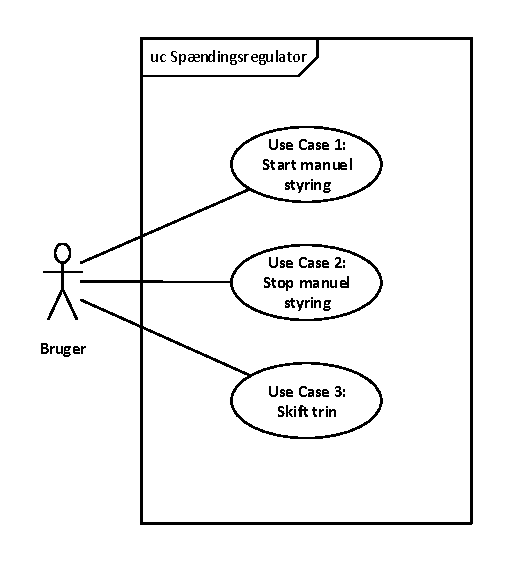
\includegraphics[width=0.5\textwidth]{figure/UsecaseDiagram}
	\caption{Usecase Diagram}
	\label{fig:UsecaseDiagram}
\end{figure}

\subsubsection{Beskrivelse af automatisk mode}
Automatisk mode funktionen overvåger spændingen ved forbrugeren og skifter trin på trintransformeren, hvis spændingen falder/stiger med 10\%. 
\begin{figure}[H] % (alternativt [H])
	\centering
	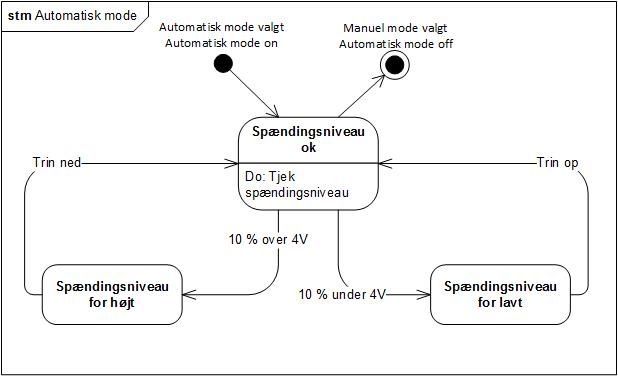
\includegraphics[width=0.8\textwidth]{figure/STM}
	\caption{Beskrivelse af automatisk mode}
	\label{fig:autoSTM}
\end{figure}